\documentclass[unknownkeysallowed]{beamer}\usepackage[]{graphicx}\usepackage[]{color}
%% maxwidth is the original width if it is less than linewidth
%% otherwise use linewidth (to make sure the graphics do not exceed the margin)
\makeatletter
\def\maxwidth{ %
  \ifdim\Gin@nat@width>\linewidth
    \linewidth
  \else
    \Gin@nat@width
  \fi
}
\makeatother

\definecolor{fgcolor}{rgb}{0.345, 0.345, 0.345}
\newcommand{\hlnum}[1]{\textcolor[rgb]{0.686,0.059,0.569}{#1}}%
\newcommand{\hlstr}[1]{\textcolor[rgb]{0.192,0.494,0.8}{#1}}%
\newcommand{\hlcom}[1]{\textcolor[rgb]{0.678,0.584,0.686}{\textit{#1}}}%
\newcommand{\hlopt}[1]{\textcolor[rgb]{0,0,0}{#1}}%
\newcommand{\hlstd}[1]{\textcolor[rgb]{0.345,0.345,0.345}{#1}}%
\newcommand{\hlkwa}[1]{\textcolor[rgb]{0.161,0.373,0.58}{\textbf{#1}}}%
\newcommand{\hlkwb}[1]{\textcolor[rgb]{0.69,0.353,0.396}{#1}}%
\newcommand{\hlkwc}[1]{\textcolor[rgb]{0.333,0.667,0.333}{#1}}%
\newcommand{\hlkwd}[1]{\textcolor[rgb]{0.737,0.353,0.396}{\textbf{#1}}}%
\let\hlipl\hlkwb

\usepackage{framed}
\makeatletter
\newenvironment{kframe}{%
 \def\at@end@of@kframe{}%
 \ifinner\ifhmode%
  \def\at@end@of@kframe{\end{minipage}}%
  \begin{minipage}{\columnwidth}%
 \fi\fi%
 \def\FrameCommand##1{\hskip\@totalleftmargin \hskip-\fboxsep
 \colorbox{shadecolor}{##1}\hskip-\fboxsep
     % There is no \\@totalrightmargin, so:
     \hskip-\linewidth \hskip-\@totalleftmargin \hskip\columnwidth}%
 \MakeFramed {\advance\hsize-\width
   \@totalleftmargin\z@ \linewidth\hsize
   \@setminipage}}%
 {\par\unskip\endMakeFramed%
 \at@end@of@kframe}
\makeatother

\definecolor{shadecolor}{rgb}{.97, .97, .97}
\definecolor{messagecolor}{rgb}{0, 0, 0}
\definecolor{warningcolor}{rgb}{1, 0, 1}
\definecolor{errorcolor}{rgb}{1, 0, 0}
\newenvironment{knitrout}{}{} % an empty environment to be redefined in TeX

\usepackage{alltt}

\usetheme{default}
\useoutertheme{infolines}
\setbeamertemplate{navigation symbols}{} 
\setbeamertemplate{footline}[frame number]
\setbeamertemplate{headline}{}

\usepackage{statrep}
\usepackage{parskip,xspace}
\newcommand*{\Statrep}{\mbox{\textsf{StatRep}}\xspace}
\newcommand*{\Code}[1]{\texttt{\textbf{#1}}}
\newcommand*{\cs}[1]{\texttt{\textbf{\textbackslash#1}}}
\setcounter{secnumdepth}{0}
\def\SRrootdir{.}
\def\SRmacropath{./statrep_macros.sas}
\usepackage[utf8]{inputenc}
\DeclareUnicodeCharacter{00D7}{$\times$}
\usepackage{graphicx}
\usepackage{hyperref}
\usepackage{multicol}
\usepackage{pbox}

\title{STAC32}
\subtitle{Applications of Statistical Methods}
\author{Ken Butler}
\IfFileExists{upquote.sty}{\usepackage{upquote}}{}
\begin{document}

\maketitle



\section{Some R stuff}

\frame{\sectionpage}

\begin{frame}[fragile]
  \frametitle{Preamble}
\begin{knitrout}
\definecolor{shadecolor}{rgb}{0.969, 0.969, 0.969}\color{fgcolor}\begin{kframe}
\begin{alltt}
\hlkwd{library}\hlstd{(tidyverse)}
\end{alltt}


{\ttfamily\noindent\itshape\color{messagecolor}{\#\# Loading tidyverse: ggplot2\\\#\# Loading tidyverse: tibble\\\#\# Loading tidyverse: tidyr\\\#\# Loading tidyverse: readr\\\#\# Loading tidyverse: purrr\\\#\# Loading tidyverse: dplyr}}

{\ttfamily\noindent\itshape\color{messagecolor}{\#\# Conflicts with tidy packages ----------------------------------------------}}

{\ttfamily\noindent\itshape\color{messagecolor}{\#\# filter(): dplyr, stats\\\#\# lag():\ \ \ \ dplyr, stats}}\end{kframe}
\end{knitrout}
\end{frame}


\begin{frame}[fragile]{Reading the data}

\begin{knitrout}\footnotesize
\definecolor{shadecolor}{rgb}{0.969, 0.969, 0.969}\color{fgcolor}\begin{kframe}
\begin{alltt}
\hlstd{jumping}\hlkwb{=}\hlkwd{read_delim}\hlstd{(}\hlstr{"/folders/myfolders/jumping.txt"}\hlstd{,}\hlkwc{delim}\hlstd{=}\hlstr{" "}\hlstd{)}
\end{alltt}


{\ttfamily\noindent\itshape\color{messagecolor}{\#\# Parsed with column specification:\\\#\# cols(\\\#\#\ \  group = col\_character(),\\\#\#\ \  density = col\_integer()\\\#\# )}}\begin{alltt}
\hlkwd{glimpse}\hlstd{(jumping)}
\end{alltt}
\begin{verbatim}
## Observations: 30
## Variables: 2
## $ group   <chr> "Highjump", "Highjump", "Highjump", "Highjump", "Highj...
## $ density <int> 650, 622, 626, 626, 631, 622, 643, 674, 643, 650, 611,...
\end{verbatim}
\end{kframe}
\end{knitrout}
\end{frame}

\begin{frame}[fragile]{A boxplot}
  
\begin{knitrout}
\definecolor{shadecolor}{rgb}{0.969, 0.969, 0.969}\color{fgcolor}\begin{kframe}
\begin{alltt}
\hlkwd{ggplot}\hlstd{(jumping,}\hlkwd{aes}\hlstd{(}\hlkwc{x}\hlstd{=group,}\hlkwc{y}\hlstd{=density))}\hlopt{+}\hlkwd{geom_boxplot}\hlstd{()}
\end{alltt}
\end{kframe}
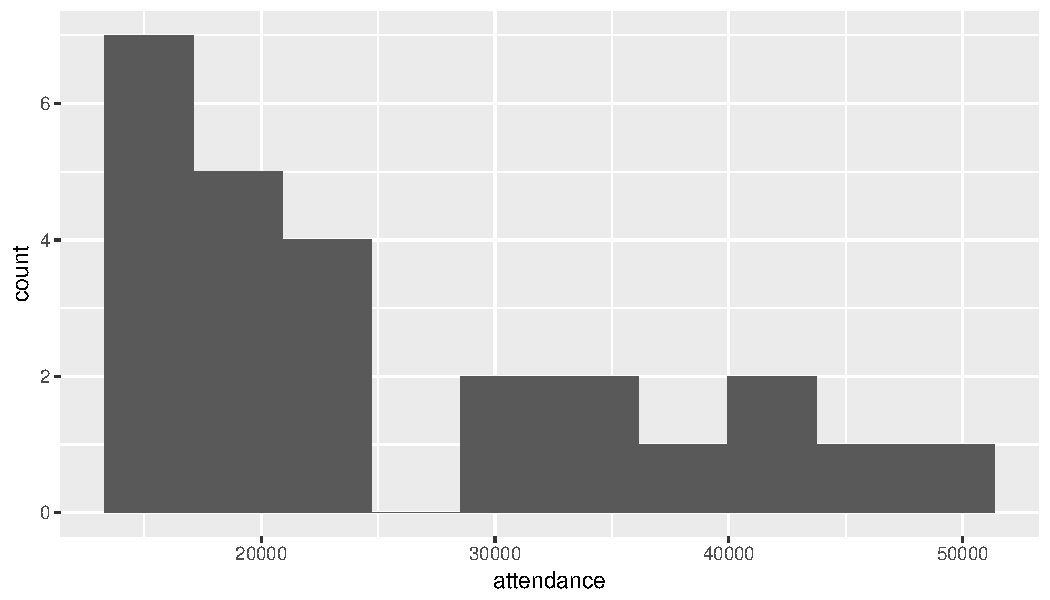
\includegraphics[width=\maxwidth]{figure/unnamed-chunk-3-1} 

\end{knitrout}
  
\end{frame}

\begin{frame}[fragile]{Mean density by group}
  
\begin{knitrout}
\definecolor{shadecolor}{rgb}{0.969, 0.969, 0.969}\color{fgcolor}\begin{kframe}
\begin{alltt}
\hlstd{jumping} \hlopt
  \hlkwd{group_by}\hlstd{(group)} \hlopt
  \hlkwd{summarize}\hlstd{(}\hlkwc{m}\hlstd{=}\hlkwd{mean}\hlstd{(density),} \hlkwc{sd}\hlstd{=}\hlkwd{sd}\hlstd{(density))}
\end{alltt}
\begin{verbatim}
## # A tibble: 3 × 3
##      group     m       sd
##      <chr> <dbl>    <dbl>
## 1  Control 601.1 27.36360
## 2 Highjump 638.7 16.59351
## 3  Lowjump 612.5 19.32902
\end{verbatim}
\end{kframe}
\end{knitrout}
  
\end{frame}


\section{The same thing in SAS}

\frame{\sectionpage}

\begin{frame}[fragile]{and now in SAS}
  
Read in data:  
  
\begin{Datastep}
proc import
  datafile='/folders/myfolders/jumping.txt'
    dbms=dlm
    out=rats
    replace;
  delimiter=' ';
  getnames=yes;
\end{Datastep}
%$ %$ %$  
  
\end{frame}

\begin{frame}[fragile]{The dataset}
  
  \begin{Sascode}[store=ac]
    proc print;
  \end{Sascode}
  
\Listing[store=ac,fontsize=tiny]{acc}  
  
\end{frame}

\begin{frame}[fragile]{Mean density by group}
  
\begin{Sascode}[store=aa]
proc means;
  var density;
  class group;
\end{Sascode}

\Listing[fontsize=scriptsize,store=aa]{aaa}
  
\end{frame}

\begin{frame}[fragile]{Code for boxplot}
  
  \begin{Sascode}[store=ab]
proc sgplot;
  vbox density / category=group;
  \end{Sascode}
  
\end{frame}

\begin{frame}[fragile]{The boxplot}
  
\Graphic[store=ab,scale=0.5]{abb}  
  
\end{frame}

\end{document}
